\subsection{Overview and Conceptual Framework}
\label{principles-overview}

After the goal of manifold learning has been formalized, it shall now be laid 
out how the problem is approached by LLE as the conceptual parent of SSLLE 
(the incorporation of prior information is a rather different matter that will 
be addressed in chapter \ref{sslle}). 
Much of the theoretical foundation for LLE has been discussed only in later 
work.
In order to provide a more integrated background, explanations will therefore be 
given in a broader context of local graph-based manifold learning, which also 
comprises LEM and HLLE.
The particular relationship of the three methods shall be made clear along the 
way.

Local graph-based manifold learning arises from a variety of geometric 
intuitions and computational implementations.
Nonetheless, methods share common structures that allow for interpretation in a 
more abstract framework (\citet{bengioetal2003}, \citet{bengioetal2004}).
It should be noted that such a framework might be established from several 
angles; after all, the different methods attempt to solve the same problem 
and can thus often be translated into one another.

Figure \ref{fig:models-overview} depicts a schematic overview on the models 
studied here, representing the specific perspective taken within this report.
All of these belong to the realm of \textit{spectral} models.
The non-spectral group includes, for instance, techniques based on neural 
networks and is not discussed here \citep{vandermaatenetal2009}.

\begin{figure}[H]
    \centering
    % https://docs.google.com/drawings/d/1982RyrkrJzhR-LHvR3xUmuCMEdpiK8qkm00HBvKMY9I/edit
    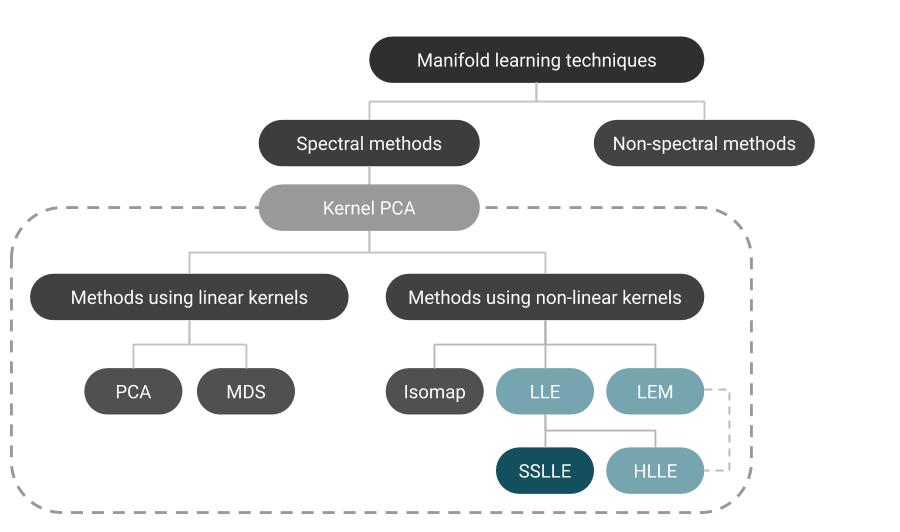
\includegraphics[trim = 0 0 0 0, clip, % left bottom right top
      width = \textwidth]{figures/models-overview}
    \caption[Overview on selected manifold learning models]{A schematic overview 
    on selected methods of manifold learning (the list is by no means extensive 
    and could arguably be ordered in several alternative ways). 
    \textit{Source:} own representation, inspired by a similar example given in 
    \citet{vandermaatenetal2009} and re-interpreted with the findings in 
    \citet{bengioetal2004}.}
    \label{fig:models-overview}
  \end{figure}

As visually indicated in figure \ref{fig:models-overview} , this report will 
sketch the idea behind local graph-based manifold learning in the light of 
\textit{kernel principal component analysis (kernel PCA)}.
Kernel PCA was actually proposed first and later shown to link the other 
concepts by a unified idea (\citet{hametal2003},
It makes for an appealing framework that, firstly, provides a useful general 
intuition to manifold learning, and, secondly, subsumes the other methods in a 
way that proves beneficial for the important task of out-of-sample extension \citep{bengioetal2004}.
\\

\textbf{Kernel PCA.} Kernel PCA builds upon two fundamental concepts 
in machine learning: it performs \textit{principal component analysis (PCA)} on 
data transformed by the \textit{kernel trick}.
In principle, it undertakes two subsequent steps.
First, features of interest are extracted from the data by kernelization. 
These are taken to capture the intrinsic data structure and may therefore be 
understood as an approximation to the latent manifold properties.
In the end, they constitute a matrix representation.
Second, \textit{principal component analyis (PCA)} finds the principal axes 
along which these intrinsic properties vary, yielding the desired reduction in 
dimensionality by preserving the most relevant latent dimensions \citep{schoelkopfetal1998}.

\begin{itemize}

  \item[] \textbf{Kernelization.} By kernelization, i.e., mapping the data to a 
  space $\mathcal{F}$ of arbitrarily high dimension, features may be obtained 
  that relate to the input in a possibly non-trivial way\footnote{
  Support vector machines use the kernel trick to achieve linear separability. 
  An intuitive example may be given by data observed in two classes that form 
  concentric circles in $\R^2$. 
  While such data are not linearly separable in two dimensions, they are in three: 
  mapping the classes to different heights enables separation by a horizontal 
  hyperplane.
  This example also hints at the idea of (spectral) clustering to which kernel 
  PCA is indeed intimately related \citep{bengioetal2004}.
  }.
  Crucially, the feature map $\phi: \RD \rightarrow \mathcal{F}$ need not be 
  computed explicitly (this might prove prohibitively expensive).
  Kernelization instead solely relies on inner products $\langle \phi(\x_i), 
  \phi(\x_j) \rangle$ of the transformed inputs.
  Employing Mercer's theorem of functional analysis, these inner products may 
  be interpreted as performed by a continuous kernel 
  % Remove domain and co-domain of kappa, might be wrong, needs the Hilbert 
  % space after all, right
  $\kappa(\x_i, \x_j)$ in some space with Hilbert property.
  Appropriate choice of $\kappa$ then allows for the data to be represented by a 
  matrix $K \in \R^{N \times N}, K_{ij} = \kappa(\x_i, \x_j)$.
  This matrix is the numerical data representation derived with respect to their 
  latent properties. \citep{schoelkopfetal1998}.
  Precisely how it is computed depends on the choice of the kernel function 
  $\kappa$ and gives rise to different techniques \citep{hametal2003}.
  
  \item[] \textbf{PCA.} PCA is a quite powerful technique by itself.
  It finds the directions of maximum variance through eigenanalysis of the 
  empirical covariance matrix, yielding the most important axes of inter-feature 
  relations that coincide with the principal eigenvectors of the covariance 
  matrix (for comments on eigenanalysis see chapter \ref{eigenanalysis} of the 
  appendix).
  The data are projected into the linear subspace spanned by these $d$ 
  eigenvectors, thereby mapping the observations to a coordinate system given 
  by those linear feature combinations that represent the strongest 
  (co)variability.
  PCA thus performs an orthogonal input transformation that allows for 
  dimensionality reduction at minimal information loss \citep{cayton2005}.
  In kernel PCA, this eigenanalysis is implicitly performed in the feature space 
  $\mathcal{F}$.
  Algorithmically, it boils down to diagonalizing the kernel matrix $K$ 
  \citep{schoelkopfetal1998}.
 
\end{itemize}

Figure \ref{fig:spirals} attempts to visualize the idea of kernel PCA.
The original data (\textit{left}) are observed in two dimensions but clearly 
intrinsically one-dimensional, where the latent manifold feature is expressed by 
coloring. 
The kernel trick creates a non-linear map, visualized here as a projection of 
the intrinsic feature to a third coordinate axis (\textit{middle}). 
Coercing the data to this dimension as the sole axis of variation yields the 
desired one-dimensional representation (\textit{right}). 

\begin{figure}[H]
  \centering
  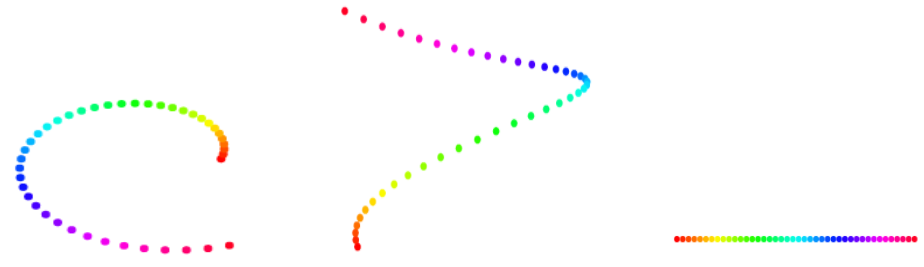
\includegraphics[width = \textwidth]{figures/spirals}
  \caption[Schematic idea of kernel PCA]{Schematic idea of kernel PCA: from data
  observed in two dimensions, but clearly of intrinsic dimensionality one 
  (\textit{left}), create a mapping to a higher-dimensional feature space 
  (\textit{middle}), reduction of which to its principal axes yields the desired 
  one-dimensional representation (\textit{right}).
  \textit{Source:} own representation, using a subset of \texttt{mlbench}'s 
  noise-free \texttt{spirals} data. Note that this is but a schematic depiction 
  where the mid and right representation have not been created by an actual 
  implementation of kernel PCA.}
  \label{fig:spirals}
\end{figure}

% ------------------------------------------------------------------------------

\subsection{Aspects of Local Graph-Based Techniques}
\label{lgb-properties}

% ------------------------------------------------------------------------------

\subsubsection{Non-Linearity and Locality}
\label{nonlin-local}

If kernel PCA sounds like a powerful concept, the crux of course lies in 
finding an appropriate kernel function.
The nature of the feature map applied to the input data determines the kind of 
mapping that may be learned and serves to distinguish the various techniques.
As foreshadowed in figure \ref{fig:models-overview}, spectral methods decompose 
into groups using \textit{linear} and \textit{non-linear} kernels, respectively.
This distinction now directly translates to the feature map $\phi$.
Linear methods suffer from the confinement to finding linear subspaces \citep{vandermaatenetal2009}.
PCA in its standard form can be interpreted as kernel PCA by identifying the 
kernel function with the covariance function.
It thus returns the subspace of greatest variability in the original input 
features \citep{hametal2003}.
The closely related \textit{multi-dimensional scaling (MDS)} approach yields the 
same result, albeit from a different intuition \citep{sauletal2006}.
\\

\textbf{Non-linearity.} As extensively discussed above, $\X$ must often be 
assumed to lie on a non-linear manifold $\mani \subset \RD$, which is precisely 
why kernelization is usually performed such that the resulting feature space is 
related to the input space in a non-linear way \citep{schoelkopfetal1998}.
Conceivably, there is no obvious way to arrive at such a mapping.
\textit{Graph-based} models therefore approach the problem from an alternative 
angle.
In fact, they do not even perform kernelization explicitly: they transform the 
data in a way that can be shown to correspond to applying a (data-dependent) 
kernel function\footnote{
The report does not discuss the actual kernel function as their illustrative 
ability is rather limited.
For an explicit formulation of kernels in LLE, LEM and HLLE see for example \citet{bengioetal2004} and \citet{weinbergeretal2004}.
}, 
but the fundamental intuition is a different one. 
The key idea in graph-based learning is to approximate the manifold by a 
discretized graph representation.
Such a graph may be intuitively imagined as a skeletal model 
of the manifold surface.
The graph properties -- essentially an approximation of the latent manifold 
properties -- are described by functionals that vary across methods.
Eigenanalysis of the associated matrix representation then leads to the 
sought-for low-dimensional subspace coordinates \citep{sauletal2006}.
\\

\textbf{Locality.} The second desideratum in general manifold learning is the 
ability to treat highly non-linear manifolds with sufficiently local focus.
Non-convexity means $\mani$ is isometric to a non-convex subset of Euclidean 
space \citep{donohogrimes2003}. 
Intuitively, such behavior requires careful tracing of the manifold surface.
Local graph-based methods therefore focus on solely local manifold properties, 
and, in doing so, produce sparse matrix representations \citep{cayton2005}.
They are frequently contrasted to \textit{Isomap}, one of the 
earliest and most prominent examples of global manifold learning.
Isomap retains pairwise distances between points on the manifold surface as 
measured along graph edges via geodesic curves\footnote{
It is thus a non-linear variant of MDS, which uses standard Euclidean distances 
\citep{tenenbaumdesilvalangford2000}.
} \citep{tenenbaumdesilvalangford2000}.
Its central assumptions are global isometry and convexity of the parameter 
space \citep{tenenbaumdesilvalangford2000}.
While it yields good results in many applications, Isomap does not sufficiently 
account for the curvature of strongly non-convex manifolds.
In order to avoid this drawback, local methods limit isometry to only hold 
between neighboring points and relax the parameter space 
condition to open, connected subspaces \citep{donohogrimes2003}.

% ------------------------------------------------------------------------------

\subsubsection{Neighborhood Graphs}
\label{algo-common}

Besides the joint framework, LLE, LEM and HLLE also share algorithmic 
commonalities, which extend to SSLLE.
The generic algorithm might be summarized as follows \citep{bengioetal2003}:

\begin{tight_enumerate}
  \item Construct a neighborhood graph $\mathcal{G}$ from the observed data.
  \item Analyze the graph properties with an appropriate functional and derive 
  a matrix representation $M$ thereof.
  \item Find the eigenvalues and associated eigenvectors of $M$.
  \item From the principal (top or bottom) eigenvectors, as determined by the 
  ordered eigenvalues, retrieve the low-dimensional coordinates.
\end{tight_enumerate}

\textbf{Neighborhoods.} All local graph-based methods fundamentally 
build on neighborhood graph approximations of the manifold surface.
A neighborhood of $\x \in \X$ is a subset of $\X$ containing another, open 
subset of $\X$ of which $\x$ is an element.
Members of the neighborhood are called neighbors of $\x$.
In metric spaces neighborhoods are defined via distances and therefore 
translate to open balls around each point \citep{waldmann2014}.
This distance-based construction locally applies to manifolds as a direct 
consequence of their local isometry to the Euclidean observation space 
\citep{mafu2011}.
There are two principal ways to build a neighborhood around $\x \in \X$, 
both of which usually employ the squared Euclidean norm\footnote{
In principle, alternative metrics are equally applicable, for instance such 
that measure angles \citep{belkinniyogi2004}.
} $\| \cdot \|^2$.
Let $\mathcal{N}: \X \rightarrow \X^{\ell}, \x \mapsto \mathcal{N} (\x)$ be a 
constructor that assigns a set of neighbors to $\x$.
The first possibility is to restrict the size of the neighborhood to the $k$ 
points with the smallest distance to $\x$, such that
$\ell = k$ and $\mathcal{N}_k(\x) = \{\x_j \in \X: 
\| \x - \x_j \|^2 \leq \gamma\}$, with $\gamma \in \R$ being the $k$-th instance 
of ordered pairwise distances.
Alternatively, the neighborhood may be constructed by collecting all points that
have a maximum distance of $\epsilon \in \R$ to $\x$, yielding 
$\mathcal{N}_{\epsilon} (\x) = 
\{\x_j \in \X: \| \x - \x_j \|^2 \leq \epsilon\}$ and 
$\ell = |\mathcal{N}_{\epsilon} (\x)|$ \citep{heetal2005}.
Both $k$ and $\epsilon$ are hyperparameters that must be specified up-front.
Their choice reflects beliefs about the topological structure of $\mani$ -- 
smaller neighborhoods corresponding to a higher degree of non-linearity -- and 
may affect performance rather strongly \citep{sudderth2002}.
\\

\textbf{Neighborhood graphs.}
$\mani$ can now be characterized by a \textit{neighborhood 
graph} $\mathcal{G} = (\mathcal{V}, \mathcal{E})$, still assuming it is 
sampled well by $\X$. 
Inputs $\x \in \X$ form vertices $\mathcal{V}$ and edges $\mathcal{E}$ 
indicate neighborhood relations \citep{belkinniyogi2001}.
Each vertex is connected to its $k$ nearest neighbors or all points 
within $\epsilon$-radius, depending on the neighborhood definition.

\begin{minipage}[b]{0.5\textwidth}
  It is easy to see that $k$-neighborhoods are an asymmetric notion; for one 
  point to be among another's $k$ nearest neighbors the reverse need not be 
  true.
  $k$-neighborhoods therefore lead to directed graphs.
  Conversely, the $\epsilon$-distance boundary holds in both directions and 
  produces undirected graphs \citep{heetal2005}.
  Figure \ref{fig:neighbor-graph} shows how a neighborhood graph may be used as 
  an approximation for the example of the S-curve manifold.
  It was built using $k$-neighborhoods with $k = 3$.
  Note that no information on the latent manifold coordinates is required.
  For a densely sampled set of points, the graph representation yields a fairly
  good approximation of the manifold surface.
\end{minipage}
\begin{minipage}[b]{0.05\textwidth}
  \phantom{xxx}
\end{minipage}
\begin{minipage}[b]{0.45\textwidth}
  \begin{figure}[H]
    \centering
    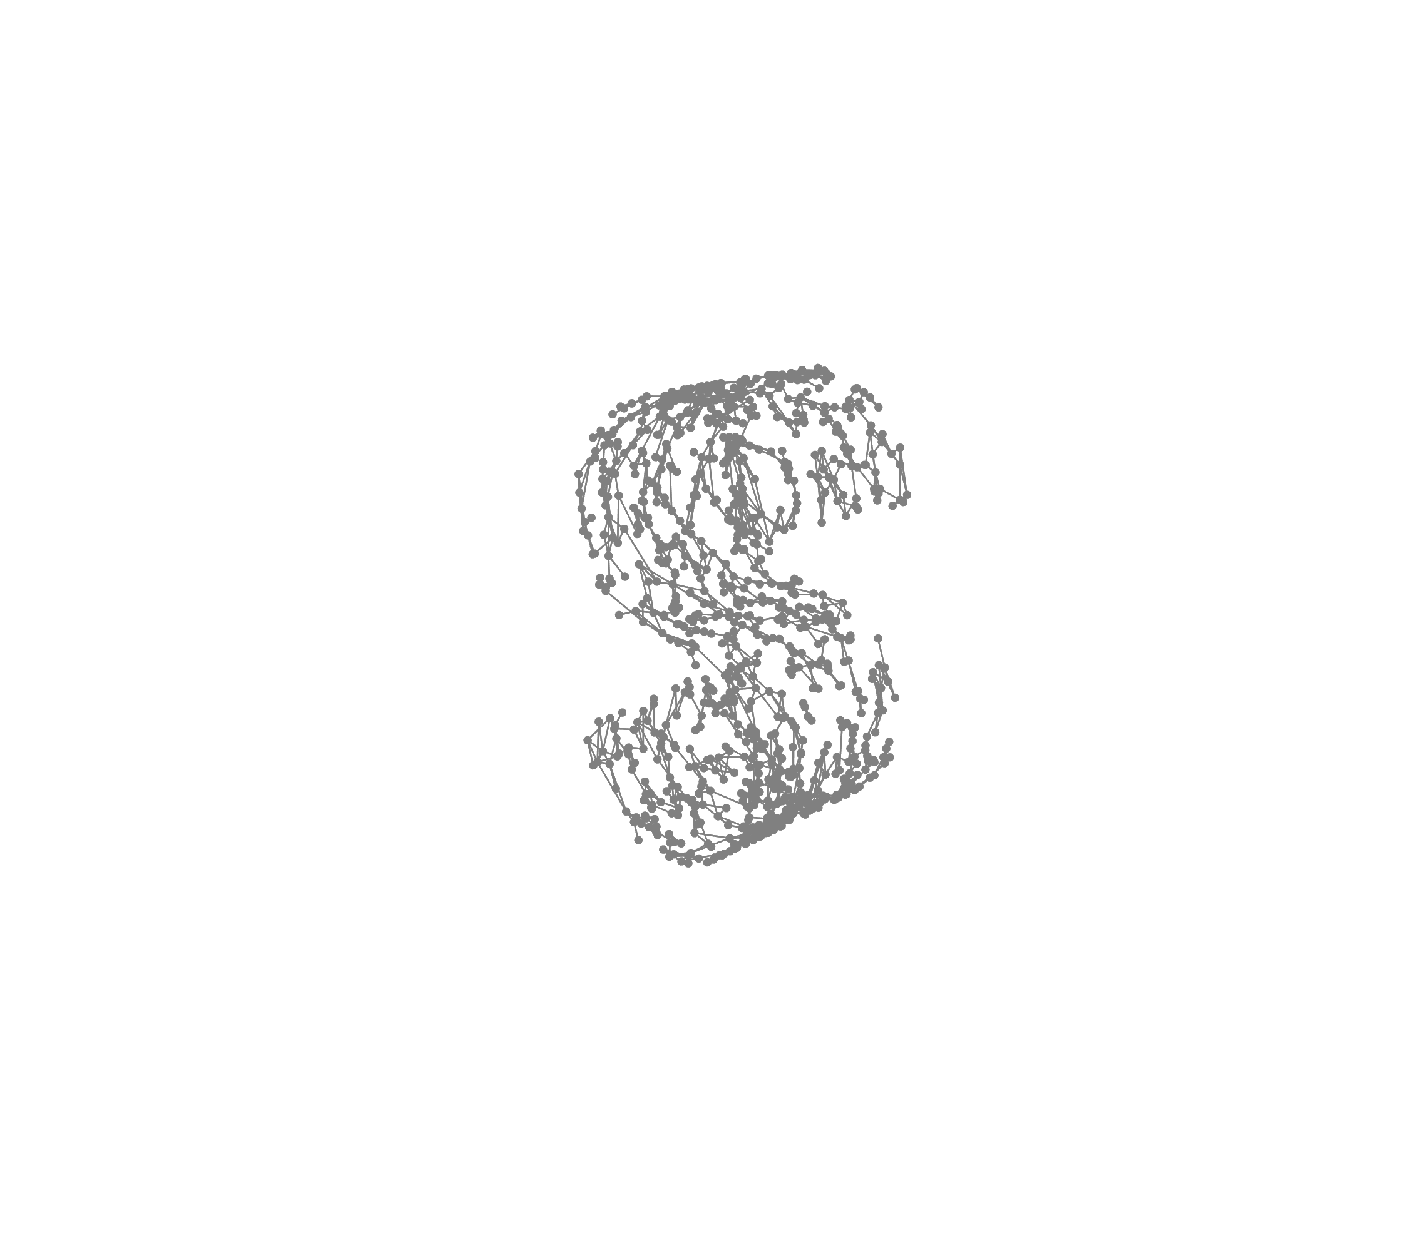
\includegraphics[trim = 250 170 200 140, clip, % left bottom right top
      width = 0.8\textwidth]{figures/s-curve-connected}
    \caption[S-curve neighborhood graph]{$k$-neighborhood graph for 300 points 
    sampled from the S-curve with $k = 5$.
    \textit{Source:} own representation.}
    \label{fig:neighbor-graph}
  \end{figure}
\end{minipage}

\textcolor{red}{Comment on difficulty of finding neighbors in high dimensions}
\\
\textcolor{red}{What about using RF proximities for neighbor search? 
Unsupervised RF works with simulating new data from the estimated dist of the 
present ones, see e.g. https://horvath.genetics.ucla.edu/html/RFclustering/RFclustering/RandomForestHorvath.pdf, https://arxiv.org/pdf/2004.02121.pdf}

% ------------------------------------------------------------------------------

\subsubsection{Challenges in Local Graph-Based Manifold Learning}
\label{challenges}

\begin{itemize}
  \item Number of neighbors
  \item Intrinsic dimensionality
\end{itemize}

% ------------------------------------------------------------------------------

\subsection{Unsupervised Techniques}
\label{techniques}

% ------------------------------------------------------------------------------

\subsubsection{Laplacian Eigenmaps (LEM)}
\label{laplace}

\begin{itemize}
  \item Notion of locality
  \item Laplacian eigenmaps
\end{itemize}

% ------------------------------------------------------------------------------

\subsubsection{Locally Linear Embedding (LLE)}
\label{lle}

\begin{itemize}
  \item Notion of local linearity
  \item Approximation of graph Laplacian
\end{itemize}

% TODO Regularized version???

% ------------------------------------------------------------------------------

\subsubsection{Hessian Locally Linear Embedding (HLLE)}
\label{hlle}

\begin{itemize}
  \item Hessian instead of Laplacian (eigenmaps)
  \item Hessian instead of LS fit (LLE)
\end{itemize}
